The results shown in this section are obtained in standard fRG using an interaction cutoff: $G_0^\Lambda = \Lambda G_0$. The calculations are performed on the Matsubara frequency axis for temperature $T=0,08 t$, where $t$ is the nearest neighbors hopping.  
The momentum dependence of the vertex is treated by means of a form factor decomposition, while keeping 29 patches in the respective bosonic momentum transfer . The critical scale is fixed by the condition that the absolute value of one of the channels exceeds a value of 1200$t$ (similar results when analyzing the suscpetibility). 
 

\begin{equation}
\label{sdmft}
a = a ;  
\end{equation}


\begin{figure}
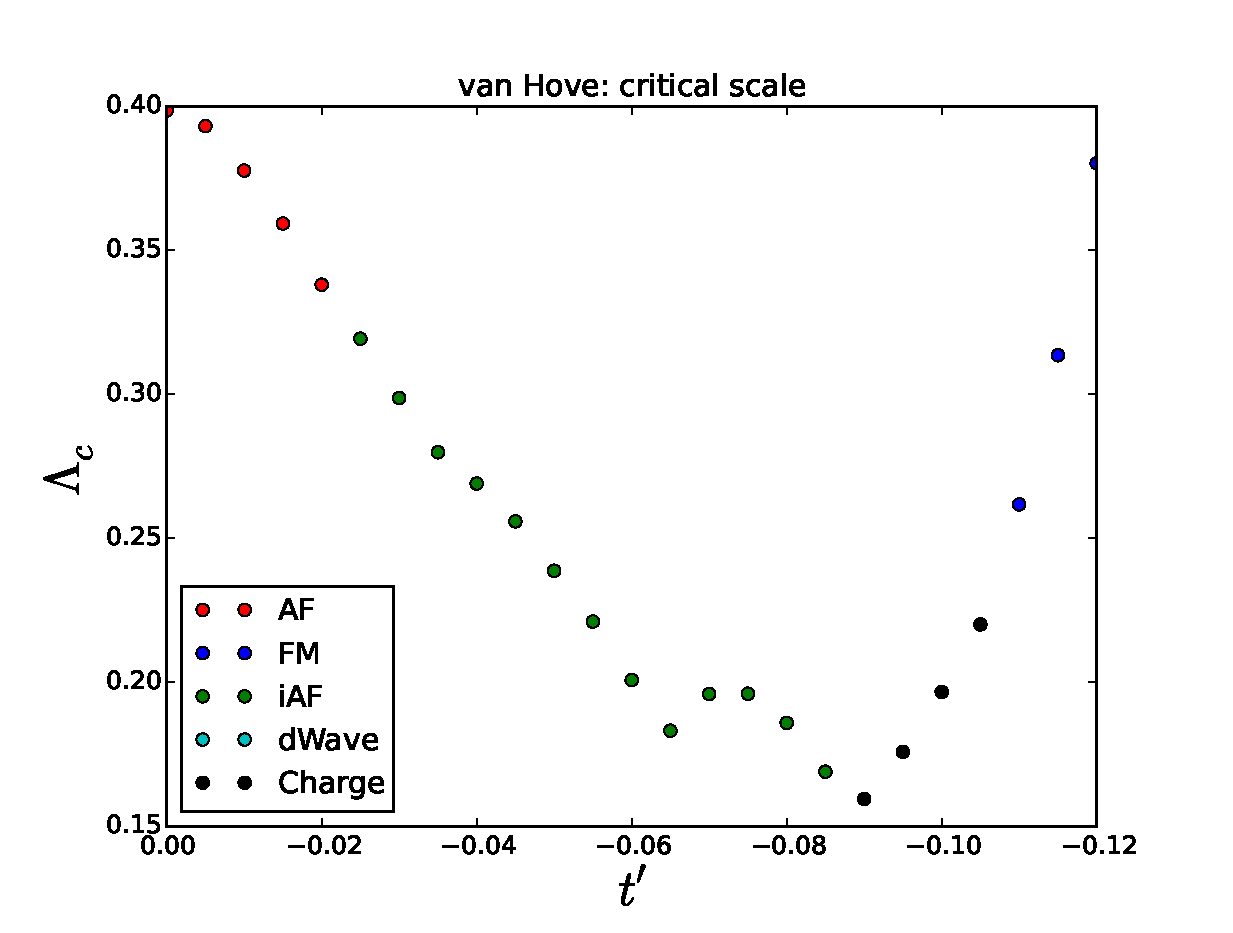
\includegraphics[scale=0.4]{vanHove_scan_critical_lambda_phi.eps}
\caption{Critical scale in full frequency fRG (interaction cutoff) as a function of the nearest neighbors hopping and for van Hove filling. The color of the symbol indicates the kind of instability that is realized.  } \label{dictionary}

\end{figure}

\begin{figure}
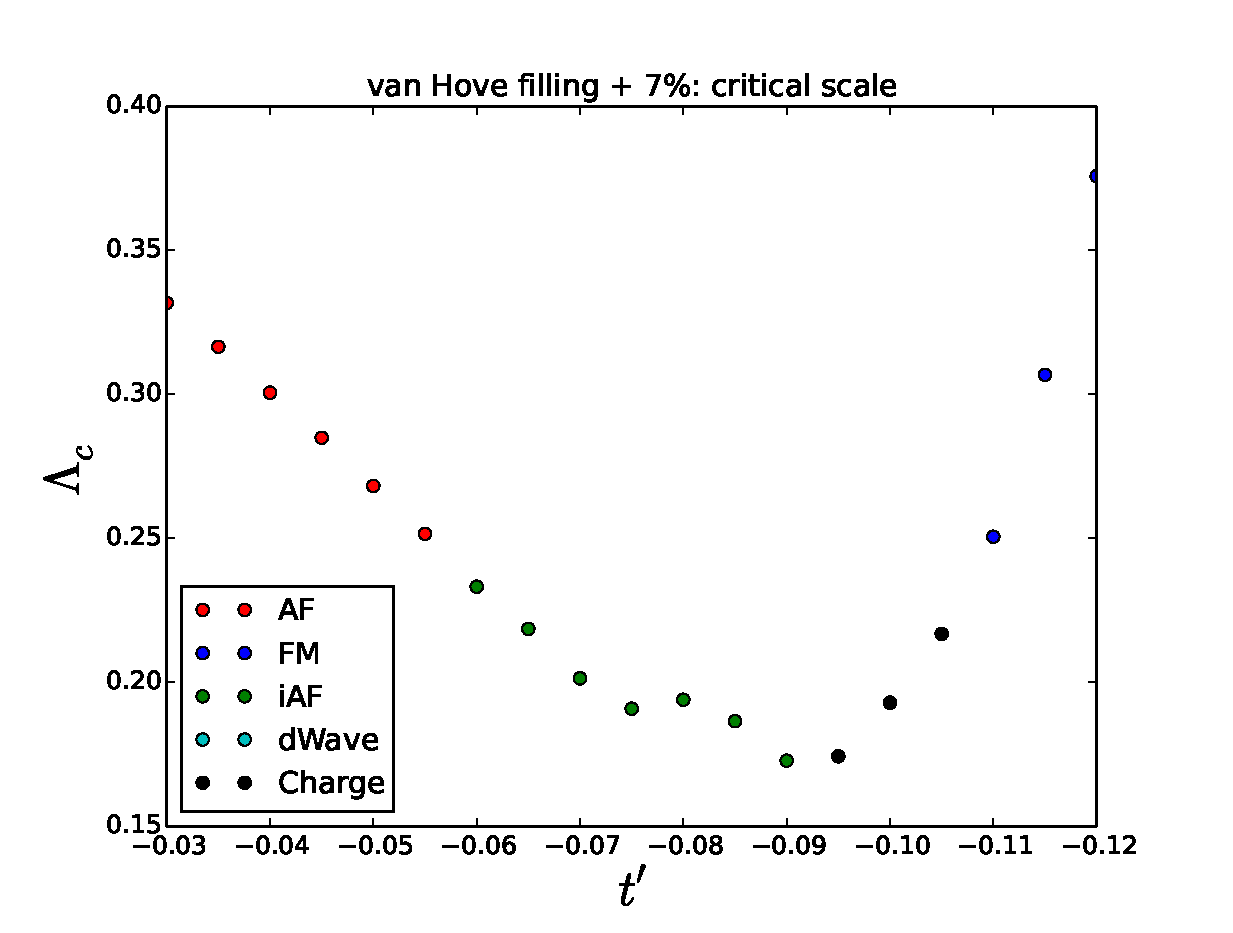
\includegraphics[scale=0.4]{vanHove_plus_scan_critical_lambda_phi.eps}
\caption{Critical scale in full frequency fRG (interaction cutoff) as a function of the nearest neighbors hopping and for van Hove filling + 7 \% . The color of the symbol indicates the kind of instability that is realized.} 
\end{figure}